\documentclass[11pt, a4paper, bibliography=totoc,listof=totoc]{scrreprt}
  \usepackage{graphicx} % Enables the inclusion of images within the document.
\usepackage{subfiles} % Allows for handling multi-file projects more easily by compiling subfiles individually.
\usepackage{nameref} % Provides commands to reference sections, figures, etc., by name instead of number.
\usepackage[T1]{fontenc} % Selects font encoding to ensure special characters are properly rendered.
%\usepackage{ngerman} % Would switch the document's language settings to German, including hyphenation patterns. It's commented out.
\usepackage{float} % Enhances the interface for defining floating objects (figures, tables) with specific placement options.
\usepackage{lipsum} % Generates filler text for document testing purposes.
\usepackage[parfill]{parskip} % Adjusts paragraph formatting to have a specific space between paragraphs instead of indentation.
\usepackage[natbibapa]{apacite} % Implements APA citation style with compatibility for the natbib citation management package.
\usepackage{setspace} % Provides commands for setting the spacing between lines in the document.
\onehalfspacing % Sets the document to use one-and-a-half line spacing.
\usepackage{mathtools} % Extends the amsmath package with improvements and bug fixes for mathematical typesetting.
\usepackage{wrapfig} % Allows figures or tables to have text wrapped around them.
\usepackage[toc,page]{appendix} % Facilitates the management of appendices, including adding them to the Table of Contents.
\usepackage[left=3cm, right=3cm]{geometry} % Adjusts the page dimensions and margins of the document.
\usepackage{enumitem} % Provides user control over the layout of lists (enumerate, itemize).
\usepackage{pdflscape} % Allows individual pages to be set in landscape mode within a PDF document.
\usepackage{csquotes} % Provides advanced facilities for inline and display quotations.
\usepackage{array} % Extends LaTeX's array and tabular environments for improved layout.
\usepackage{makecell} % Simplifies the creation of multi-lined tabular cells.
\usepackage{siunitx} % A comprehensive (SI) units package, ensuring consistent application of units.
\usepackage{fancyhdr} % Enables extensive control over page headers and footers.
\usepackage{listings} % Provides typesetting source code listings.
\usepackage{hyperref} % Provides extensive support for creating hyperlinks within the document.
\usepackage{varwidth} % Allows for variable width of boxes in the document.
\usepackage{helvet} % Sets Helvetica as the default sans-serif font.
\usepackage{caption} % Enhances the captioning capabilities of floating environments.
\usepackage{booktabs} % Facilitates the creation of publication quality tables in LaTeX.
\usepackage{siunitx} % Provides a comprehensive (SI) units package. (Duplicate)
\usepackage{csquotes} % Enhances the facilities for inline and display quotations. (Duplicate)
\usepackage{fancyhdr} % Allows for extensive customization of headers and footers. (Duplicate)
\captionsetup[table]{aboveskip=10pt} % Adjusts the space above table captions.
\usepackage[automake, nonumberlist]{glossaries} % Would provide advanced glossary features. It's commented out.
\renewcommand{\familydefault}{\sfdefault} % Changes the default font family to sans-serif.
\setlist[enumerate]{label*=\arabic*.} % Configures enumerate environments to label items with arabic numerals.
\hypersetup{ hidelinks = true, } % Configures the hyperref package to hide links for a cleaner look.


  \newcommand\frontmatter{%
\cleardoublepage
%\@mainmatterfalse
\pagenumbering{roman}}

\newcommand\mainmatter{%
\cleardoublepage
% \@mainmattertrue
\pagenumbering{arabic}}

\newcommand\backmatter{%
\if@openright
\cleardoublepage
\else
\clearpage
\fi
% \@mainmatterfalse
}

\newenvironment{enum_short}
{ \begin{enumerate}
    \setlength{\itemsep}{0pt}
    \setlength{\parskip}{0pt}
    \setlength{\parsep}{0pt}     }
{ \end{enumerate}                  } 

%\makeatletter
%\renewcommand\listoftables{%
%        \@starttoc{lot}%
%}
%\makeatother
%
%\makeatletter
%\renewcommand\listoffigures{%
%        \@starttoc{lof}%
%}
%\makeatother





\renewcommand*\chapterheadstartvskip{\vspace*{-1.5cm}}


\lstdefinestyle{mystyle}{
    backgroundcolor=\color{backcolour},   
    commentstyle=\color{codegreen},
    keywordstyle=\color{magenta},
    numberstyle=\tiny\color{codegray},
    stringstyle=\color{codepurple},
    %identifierstyle=\color{powderblue},
    basicstyle=\ttfamily\footnotesize,
    language=Bash,              % the language of the code
    breakatwhitespace=false,         
    breaklines=true,                 
    captionpos=b,                    
    keepspaces=true,                 
    numbers=left,                    
    numbersep=5pt,                  
    showspaces=false,                
    showstringspaces=false,
    showtabs=false,                  
    tabsize=2
}

\lstset{style=mystyle}


  \pagestyle{fancy}
  \fancyhf{}
  \renewcommand{\chaptermark}[1]{\markboth{#1}{#1}}
  \fancyhead[R]{}
  \fancyhead[L]{\chaptername\ \thechapter\ --\ \leftmark}
  \rfoot{Seite \thepage}
  \bibliographystyle{apacite}
  \makeglossaries

\newglossaryentry{word_embedding}{
  name=Word Embeddings,
  description={Mapping of words into vectors with real numbers}
}

\newglossaryentry{tokenization}{
  name=Tokenization,
  description={Splitting the text into individual tokens, which are the atomic units of information in a chosen language representation. English NLP models typically use words as tokens. Since proteins do not have a well-defined vocabulary of words, word-level tokenization is not a well-defined option in the case of proteins, which is why subword segmentation is often used}
}


%\newglossaryentry{multilingual}{
%  name=multilingual,
%  description={Für mehrere Sprachen einsetzbar. Im Zusammenhang mit Deep Learning wird ein multilinguales Modell oft anhand von mehreren Sprachen trainiert}
%}


  \begin{document}
    \frontmatter
    \begin{titlepage}
  \centering
  {\huge\bfseries "Heavy-Light Chain Pair Identification in Antibodies (work title)" \par}
  \vspace{2cm}
   {\scshape\LARGE Master thesis \\ Faculty of Science,  University of Bern  \par}
  \vspace{1cm}
  {\scshape\Large Handed in by \par}
  \vspace{0cm}
  {\Large \textbf{Lea Br\"{o}nnimann} \par}
  \vfill
  {\Large \scshape 2024 \par}
  \vspace{2cm}
  {\scshape\Large Supervisor: \par}
  \vspace{0cm}
  {\Large \textbf{Prof. Dr. Thomas Lemmin} \par}
  \textbf{} \par
  \vfill
  \vfill
  \textbf{} \par
   \par
 \par
  \vfill

  % Bottom of the page
 %{\large \textbf{Kirchdorf, \today}\par}
\end{titlepage}

    \chapter*{Abstract} \label{abstract}

    \tableofcontents

    \glsaddall
    \printglossary[title={Glossary}]

    \mainmatter
    \chapter{Introduction} \label{introduction}

    \chapter{Sequential Transfer Learning in NLP for Antibody Research} \label{theorie}

% A comprehensive review of existing research relevant to your topic. This section establishes the foundation on which your research is built and identifies gaps your study aims to fill.

The following section explains the theoretical background necessary for the thesis with regard to the biology of antibodies and the functionality of the NLP models used. A basic understanding of machine learning and protein structures is assumed.

\section{Introduction to Antibodies}

% Basic Immunology Concepts: Overview of the immune system, with a focus on the structure and function of antibodies. Antibody Diversity: Discuss how diversity is generated in antibody populations, emphasizing the significance of heavy and light chains.

Antibodies are Y-shaped proteins that consist of two identical light chains (LCs) and two identical heavy chains (HCs) \citep{Chiu2019}.


\section{Antibody Engineering and Therapeutic Applications}

% Overview: Introduction to the field of antibody engineering and the role of antibodies in therapeutic applications. Challenges: Discuss the challenges in identifying and pairing heavy and light chains in recombinant antibodies and their implications for therapeutic development.

\section{Deep Learning Methods for Antibody Research}

Deep learning is a branch of machine learning that focuses on algorithms capable of identifying complex patterns in data by transforming low-level inputs (like pixels in an image) into high-level features (such as object shapes). It utilizes artificial neural networks (ANNs) with multiple layers between the input and output, making them "deep". These networks consist of nodes, or neurons, that process inputs and pass the outputs to subsequent layers, gradually extracting more abstract features. In the context of biochemistry, deep learning can start from basic data, like amino acid sequences, and learn to recognize complex biological structures or functions \citep{Graves2020}. NLP models can be effectively used for analyzing amino acid sequences due to the conceptual similarities between proteins and language. Proteins can be represented as strings of 20 amino acid letters, making them a natural fit for many NLP methods. This similarity in representation allows for the application of NLP algorithms to the study of proteins, leveraging the success and promise of NLP methods in other domains \citep{Ofer2021}. NLP methods have been successfully applied to protein sequences for tasks such as predicting protein families or properties. Word embedding models in NLP have been used to extract features of protein sequences and have demonstrated successful applications in protein family classification \citep{Xu2020}. This can be explained by the following similarities between natural language and protein sequences: Like natural language, natural proteins generally consist of reused modular elements that exhibit slight variations and can be rearranged and reassembled in a hierarchical fashion. In this analogy, common protein motifs and domains, which are the basic functional building blocks of proteins, are comparable to words, phrases and sentences in human language. Another similarity between proteins and human language is the completeness of the information. A protein is more than just a sequence of amino acids, it is also a three-dimensional machine with a specific structure and associated function, which is largely determined by the amino acid sequence. From an information-theory perspective, this means that the information of the protein is contained in the protein sequence. However, the analogies between proteins and human language only go so far. We can read and understand human language, but not in the same way as the protein sequence. In addition, most human languages have uniform punctuation and stop words that clearly delineate structures such as words or sentences. There is no clear analogy between the building blocks of languages and those of proteins \citep{Ofer2021}.

\begin{figure}[h]
 \centering
 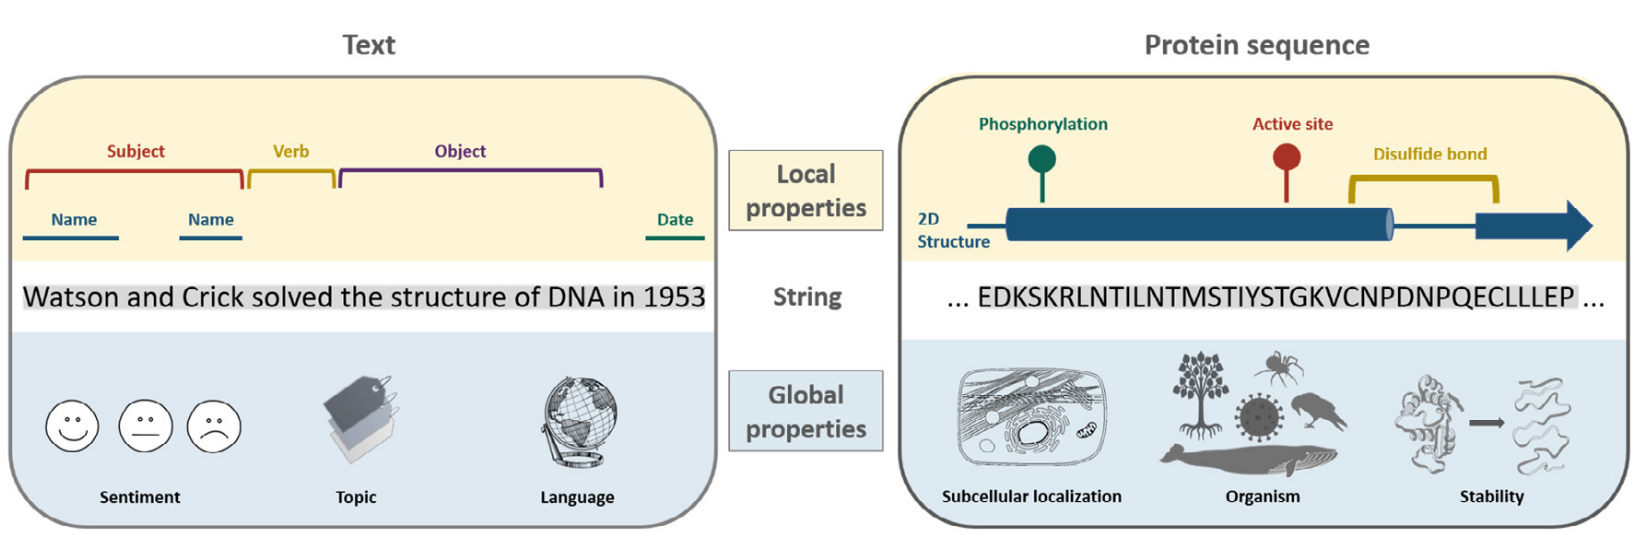
\includegraphics[width=15cm]{images/protein_representation.png}
 \caption{\citep{Ofer2021}}
 \label{protein representation}
\end{figure}

\section{BERT and Transformers in Bioinformatics}

% BERT Overview: Explain the BERT model (Bidirectional Encoder Representations from Transformers) and its significance in natural language processing (NLP). Adaptation to Bioinformatics: Discuss how BERT and transformer models have been adapted for bioinformatics applications, including examples where they have been used for sequence analysis, protein function prediction, etc.

BERT from \cite{Devlin2019} stands for "Bidirectional Encoder Representations from Transformers" and is based on a bidirectional language model. BERT uses the transformer according to \cite{Vaswani2017} as its architecture. At the time of publication, BERT was able to establish the state of the art in 11 natural language processing tasks \citep{Devlin2019}. The first forms of language modelling in connection with machine learning can be found in \cite{Mikolov2013} in the form of the "skip-gram" model. In the skip-gram model, text or unlabelled data is used to train the probability distribution of the next word based on the previous words in the sentence. This process can then be used to calculate static word vectors, which serve as a starting point for other NLP tasks \citep{Mikolov2013a}. The idea of this unidirectional language model was subsequently used by various other publications and transferred to other architectures such as the Transformer according to \cite{Vaswani2017} \citep{Radford2018ImprovingLU}. In contrast to \cite{Radford2018ImprovingLU}, however, BERT uses a bidirectional language model. Figure \ref{bert_overview} shows the structure of BERT with pretraining and fine-tuning in graphical form. The language model, or the step known as "pre-training", is trained using two tasks:

\textit{Masked language modelling}: Since the words of the sentence are processed in parallel in the transformer architecture \cite{Vaswani2017}, individual words must be masked in bidirectional prediction. In the case of BERT, these are replaced with the token "[MASK]". The model is then trained to correctly predict these masked words.

\textit{Next Sentence Prediction}: In order to encode connections between whole sentences in the language model, "Next Sentence Prediction" is used in addition to "Masked Language Modelling". For two sentences $A$ and $B$, in 50\% of the sentences, a sentence $B$ is actually used, which occurs in the text as a directly following sentence after $A$, and in 50\% of the cases a random other sentence is used, which is taken from the corpus. The model must then predict whether these sentences belong together or not.

\begin{figure}[h]
 \centering
 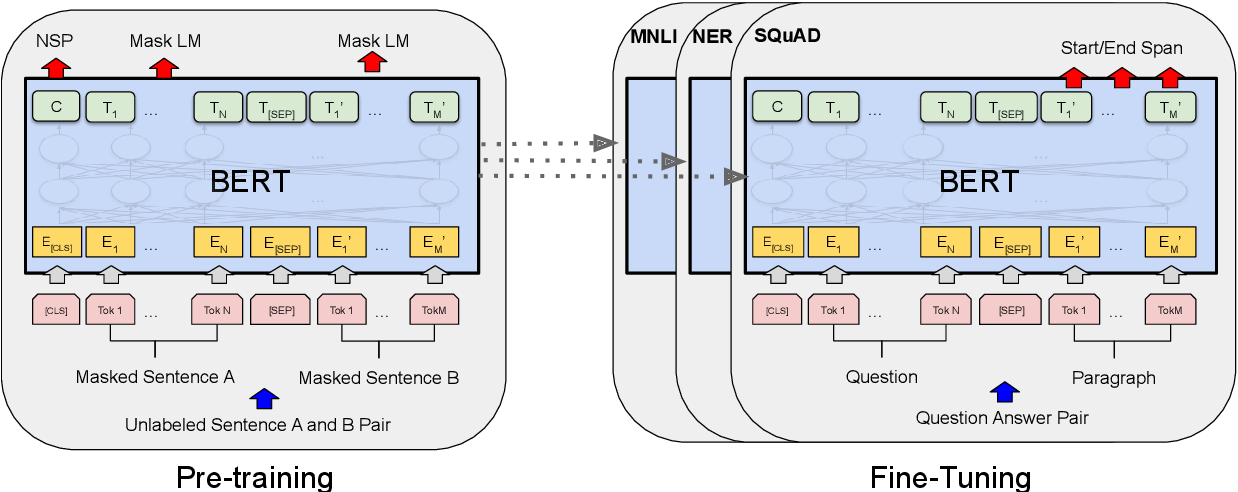
\includegraphics[width=15.5cm]{images/bert_architecture.png}
 \caption{BERT Overview \citep{Devlin2019}.}
 \label{bert_overview}
\end{figure}



\section{Heavy-Light Chain Pair Identification}

% Current Methods: Review current methods and challenges in identifying and pairing heavy and light chains in antibodies. Potential of BERT Models: Discuss the potential advantages and challenges of using BERT models for heavy-light chain pair identification, including any preliminary findings or hypotheses.


\subsection{Gap in the Literature}

% Identify the Gap: Based on your review, identify the gap in current research that your thesis aims to address. This could involve limitations in existing methods for heavy-light chain identification, or the unexplored potential of BERT models in this specific application.



\subsection{Conclusion}

% Summarize Key Points: Briefly summarize the key points from your literature review, emphasizing the importance of your research question and the potential impact of your work.


    \chapter{Materials \& Methods} \label{methoden}


    \chapter{Results} \label{resultate}



    \chapter{Discussion} \label{diskussion}



    \chapter{Conclusion}


    \bibliography{/Users/leabroennimann/Desktop/Master_Bioinformatik/master_thesis_24_LB/Master_Thesis_tex/bibtex/master_thesis_bib.bib}
    \listoffigures
    \listoftables
    
    \backmatter
    \appendix
    \chapter{Appendix}

\section{Selbstst{\"a}ndigkeitserkl{\"a}rung}

%\includepdf[]{BSc_bachelorarbeit_erklaerung_RSL18.pdf}


  \end{document}